
\documentclass[aspectratio=169]{beamer}
\usetheme{metropolis}           % Use metropolis theme
\usepackage[utf8]{inputenc}
\usepackage{graphicx}
\usepackage{eso-pic}
\usepackage{graphics}
\usepackage{tikz}
\usepackage[export]{adjustbox}
\usepackage{multicol}
\usepackage{listings}
\usepackage{helvet}
\usepackage{booktabs}
\usepackage{threeparttable}
\usepackage{upquote}

\title{Data Management for \newline Reproducible Research}
\date{\today}
\author{Benjamin Daniels} % Name of author(s) of session here
\institute{Development Impact Evaluation (DIME) \newline The World Bank }
\setbeamercolor{background canvas}{bg=white}	% Sets background color

% The below command places the World Bank logo and DIME logo to the right corner
\titlegraphic{%
	\begin{picture}(0,0)
	\put(330,-180){\makebox(0,0)[rt]{
\includegraphics[width=3cm]{img/WB_logo}}}
	\end{picture}%
	\begin{picture}(0,0)
	\put(390,-180){\makebox(0,0)[rt]{
\includegraphics[width=1.5cm]{img/i2i}}}
	\end{picture}%
}

%%% Section page with picture of Light bulb
\makeatletter
\defbeamertemplate*{section page}{mytheme}[1][]{
	\centering
	\begin{minipage}{22em}
		\raggedright
		\usebeamercolor[fg]{section title}
		\usebeamerfont{section title}
		\par
		\ifx\insertsubsectionhead\@empty\else%
		\usebeamercolor[fg]{subsection title}%
		\usebeamerfont{subsection title}%
		\fi
		\ifstrempty{#1}{}{%
			\includegraphics[width=100mm, height=60mm]{#1}%
		}
		\insertsectionhead\\[-1ex]
		\insertsubsectionhead
		\usebeamertemplate*{progress bar in section page}
		
	\end{minipage}
	\par
	\vspace{\baselineskip}
}
\makeatother

%%% Define a command to include picture in section, 
%%% make section, and revert to old template
\newcommand{\sectionpic}[2]{
	\setbeamertemplate{section page}[mytheme][#2]
	\section{#1}
	\setbeamertemplate{section page}[mytheme]
}

%%% The command below allows for the text that contains Stata code
\lstset{ %
	backgroundcolor=\color{white},
	basicstyle=\tiny,
	breakatwhitespace=false,
	breaklines=true,
	captionpos=b,
	commentstyle=\color{green},
	escapeinside={\%*}{*)},
	extendedchars=true,
	frame=single,
	numbers=left,
	numbersep=5pt,
	numberstyle=\tiny\color{gray},
	rulecolor=\color{black},
	showspaces=false,
	showstringspaces=false,
	showtabs=false,
	stringstyle=\color{mauve},
	tabsize=2,
	title=\lstname,
	morekeywords={not,\},\{,preconditions,effects },
	deletekeywords={time}
}

%% The below command creates the ligh bulb logos in the top right corner of the 
\begin{document}
	
{
	\usebackgroundtemplate{
\includegraphics[height=55mm, right]{img/top_right_corner.pdf}}
	\maketitle
}

\begin{frame}{Introduction: Data Management}
\textbf{Data management is part of a reproducible research workflow}

	\begin{itemize}[<default overlay specification>]
	\item<1>  This presentation will show you best practices to manage data work.
	\item<1>  At DIME, we have large teams collaborating on the same codes and data sets. 
	\item<1>  Long projects easily become complex, with multiple rounds of data collection to organize. 
	\item<1>  Standardizing organization of documents and code prevents mistakes and reduces the cost of transitioning across projects and teams
.
	\end{itemize}

\end{frame}

\begin{frame}

	\begin{figure}
		\centering
		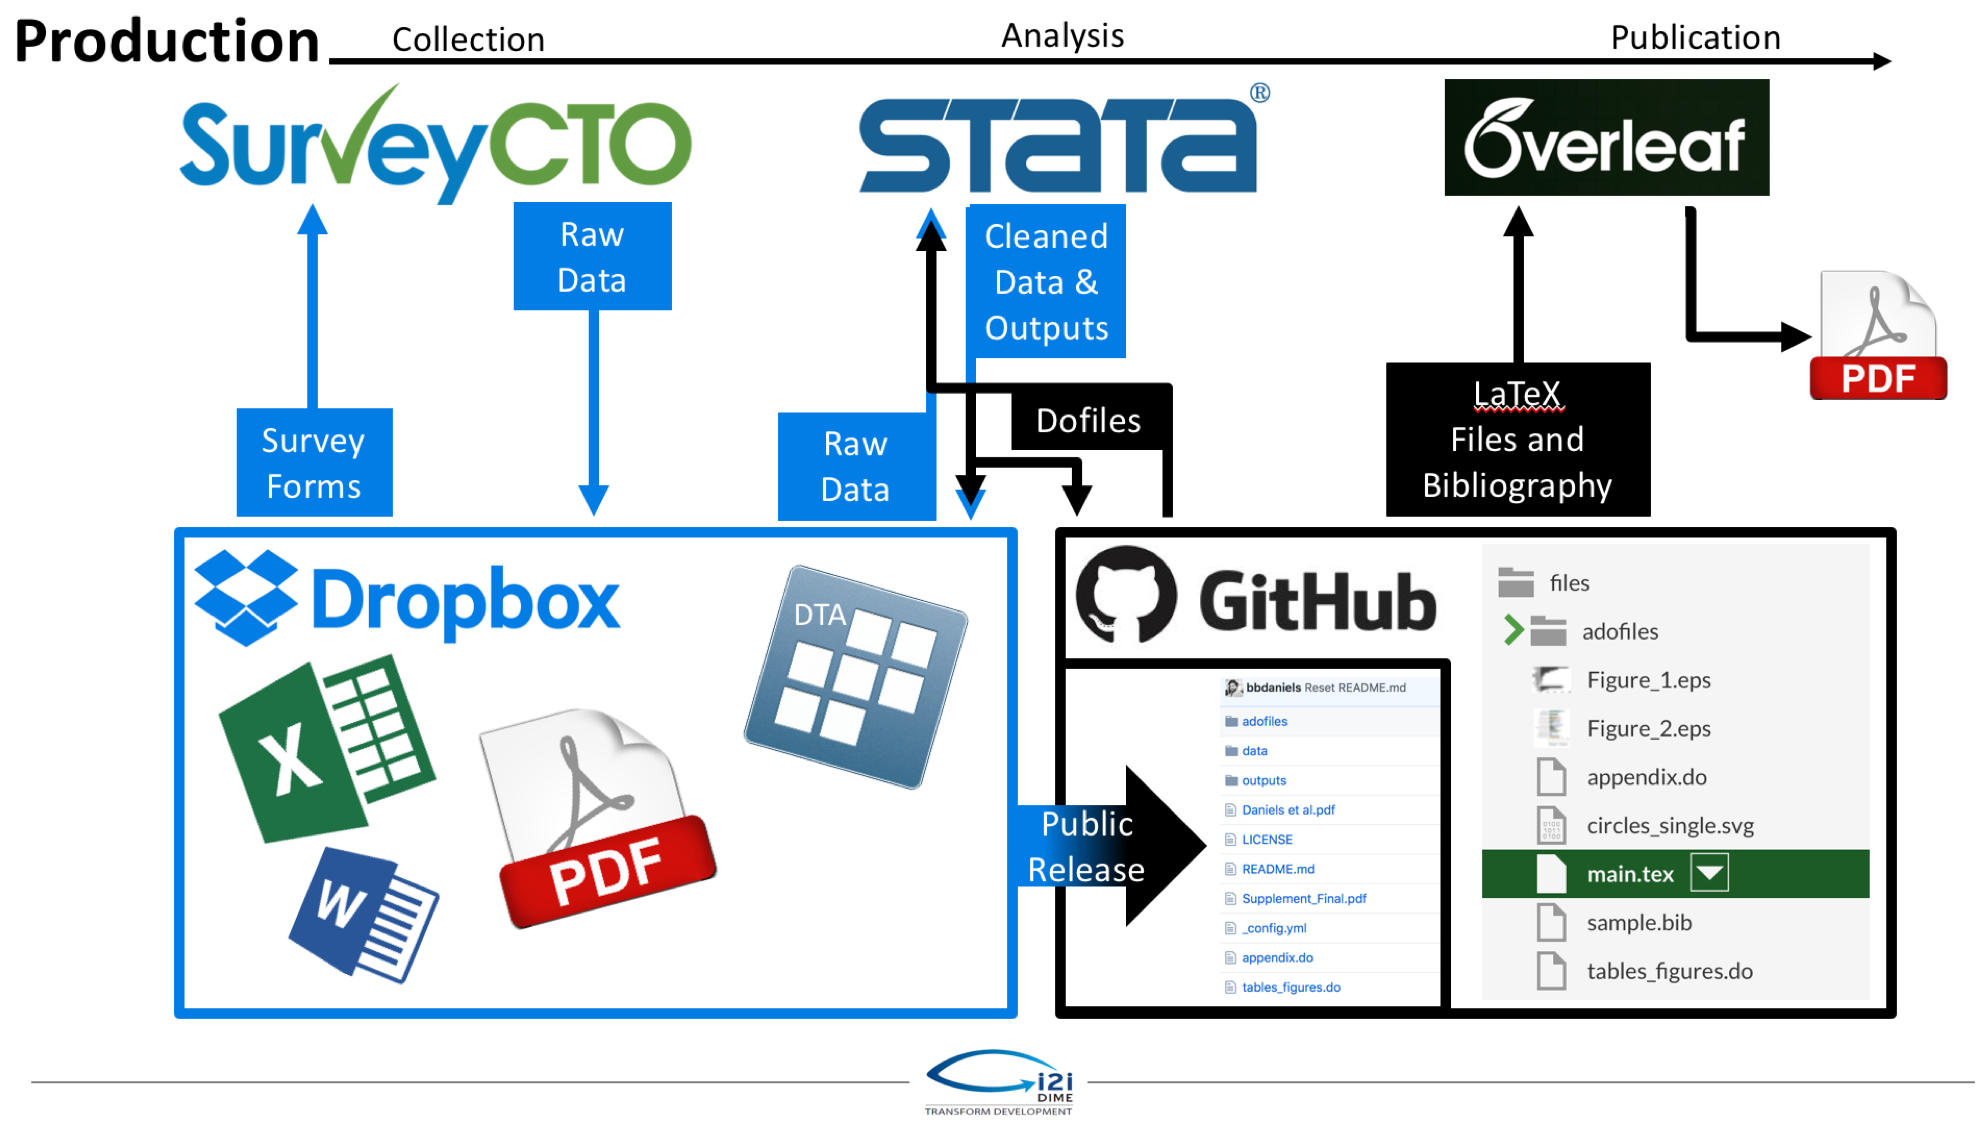
\includegraphics[width=\linewidth]{img/Production}
	\end{figure}

\end{frame}

\begin{frame}

	\begin{figure}
		\centering
		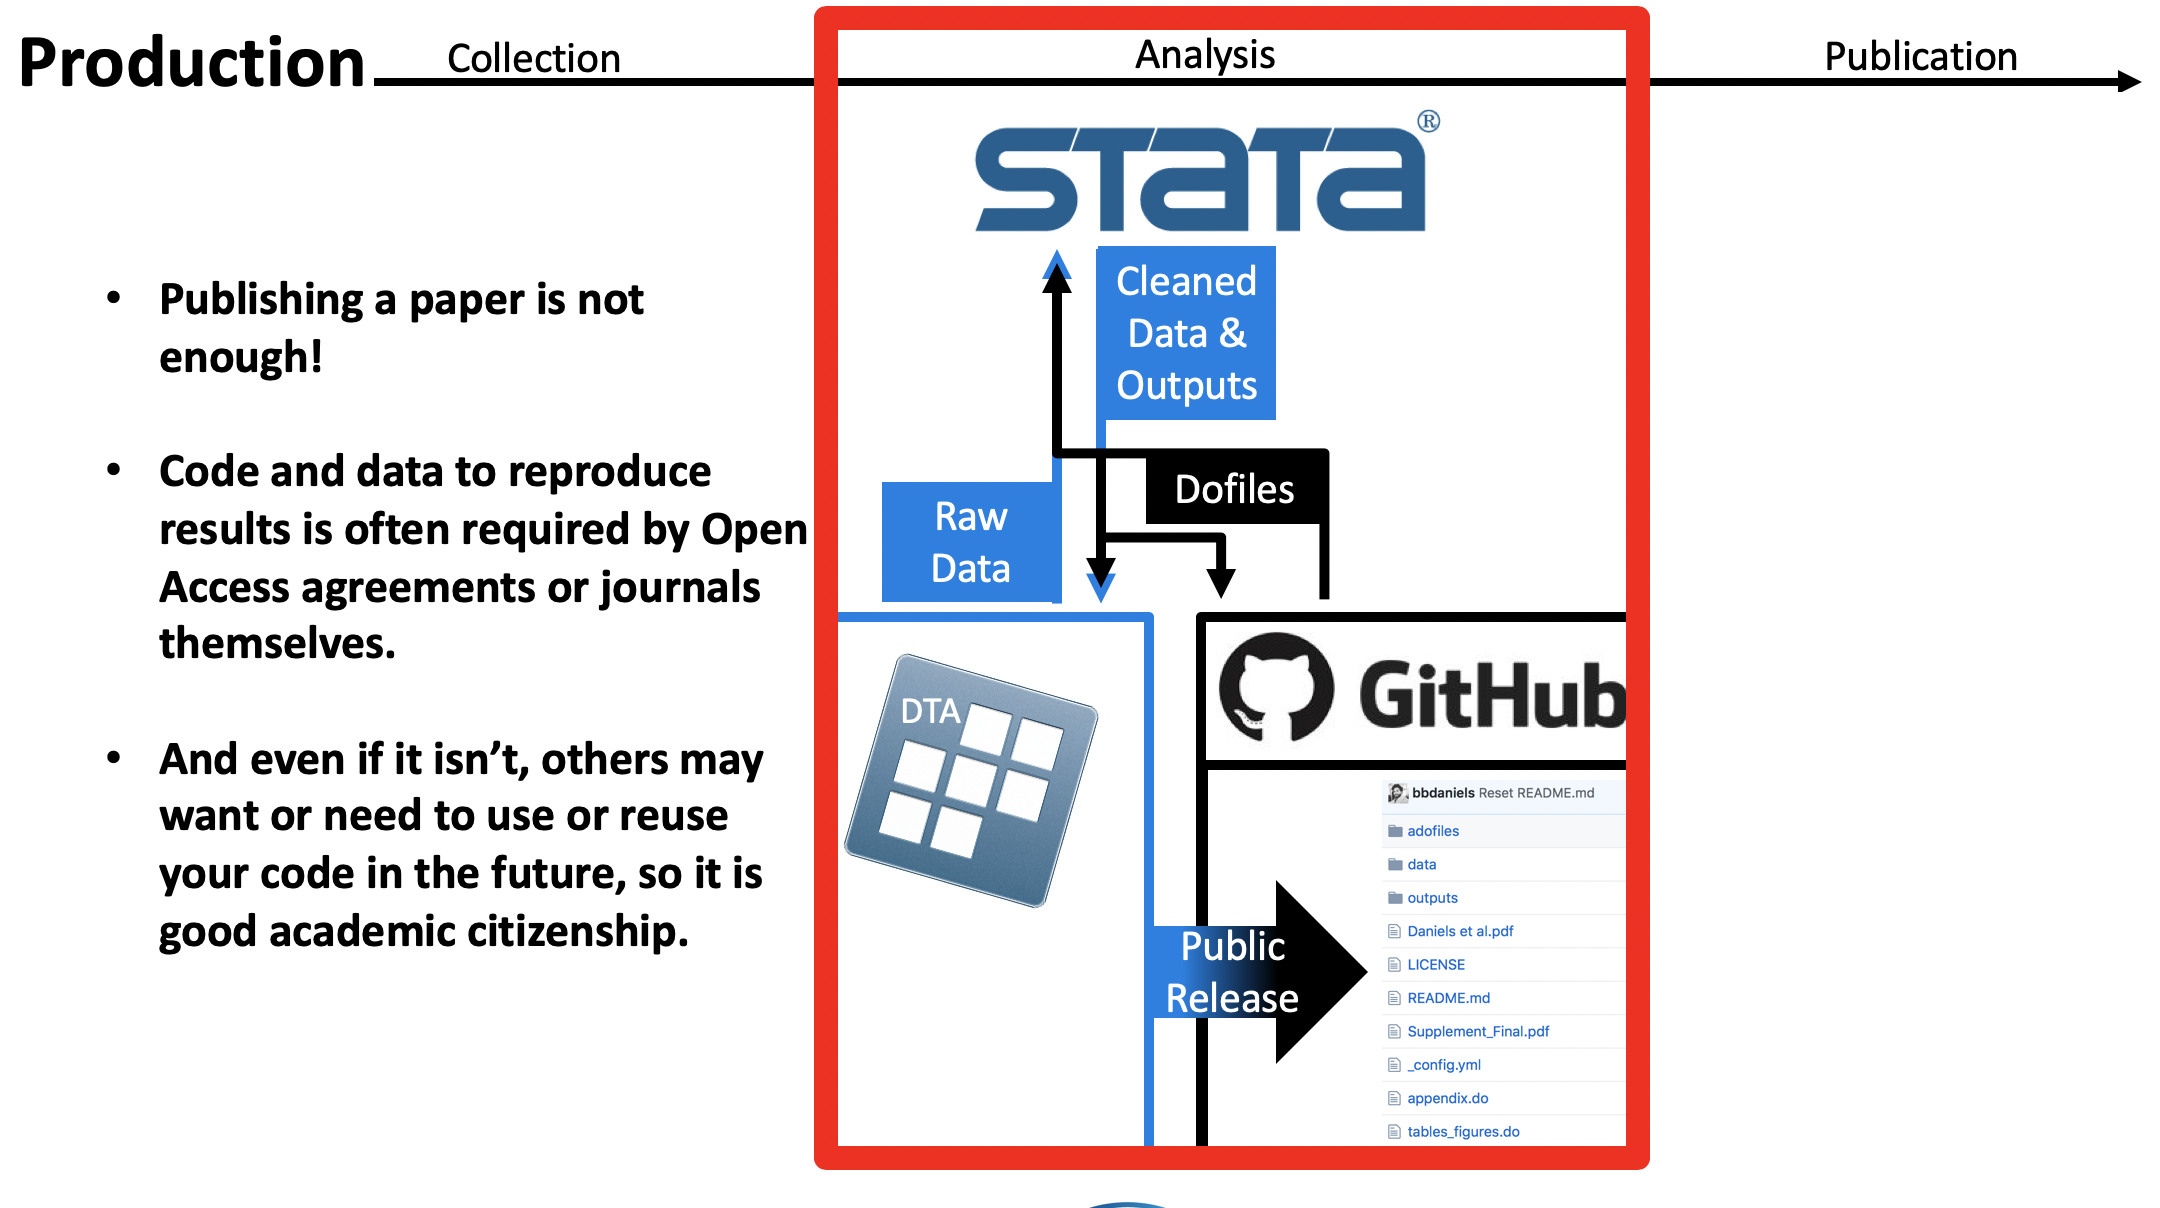
\includegraphics[width=\linewidth]{img/Production2}
	\end{figure}

\end{frame}


\begin{frame}[fragile]{Organized code requires organized data}
\begin{multicols}{2}	
	
	By the end of this presentation, you should understand how these two are connected in a research workflow:
	
	\begin{itemize}[<default overlay specification>]
		\item<1>The structure of the folder where the data work is stored.
		\item<1> The master do-file for a project’s data work.
	\end{itemize}
	
	\begin{figure}
		\centering
		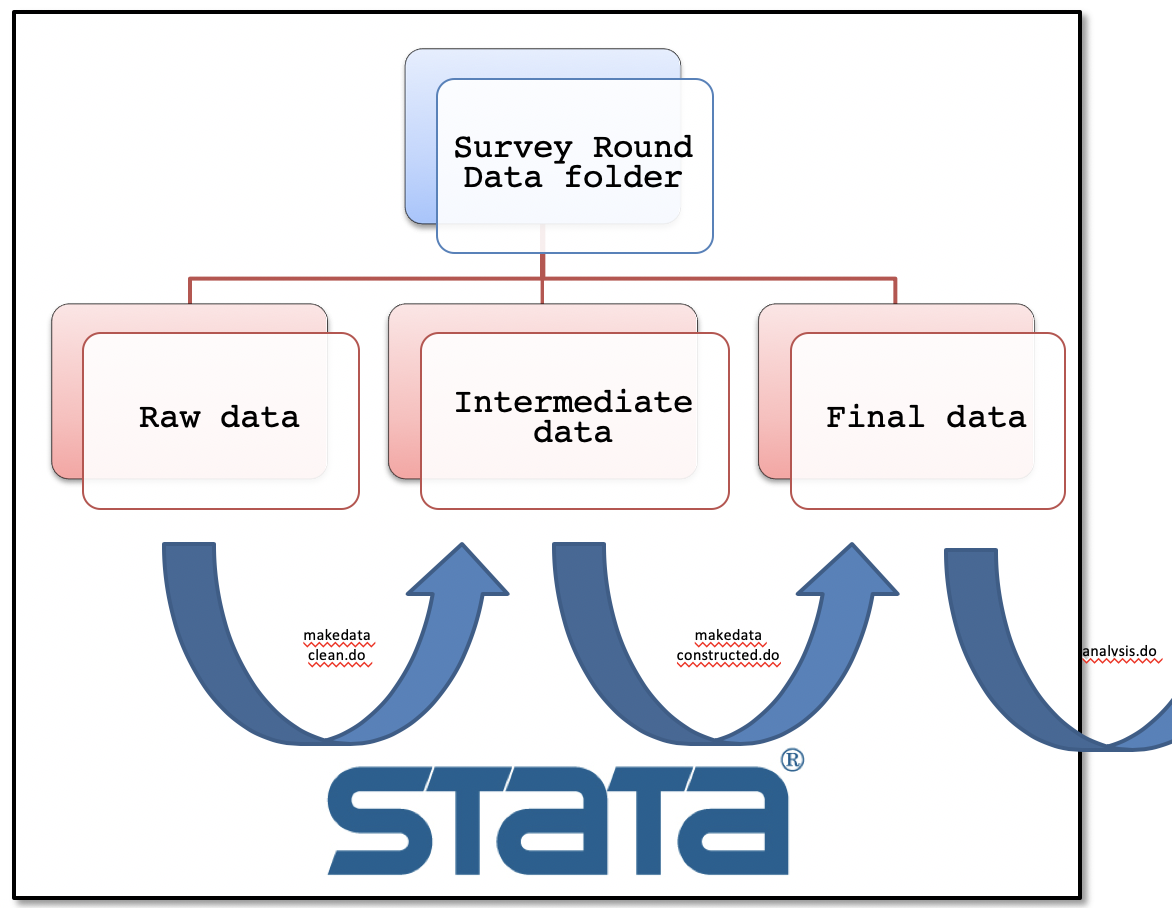
\includegraphics[width=50mm]{img/Organize}
	\end{figure}
	
\end{multicols}
\end{frame}

\begin{frame}{What does this look like in practice?}

	\begin{figure}
		\centering
		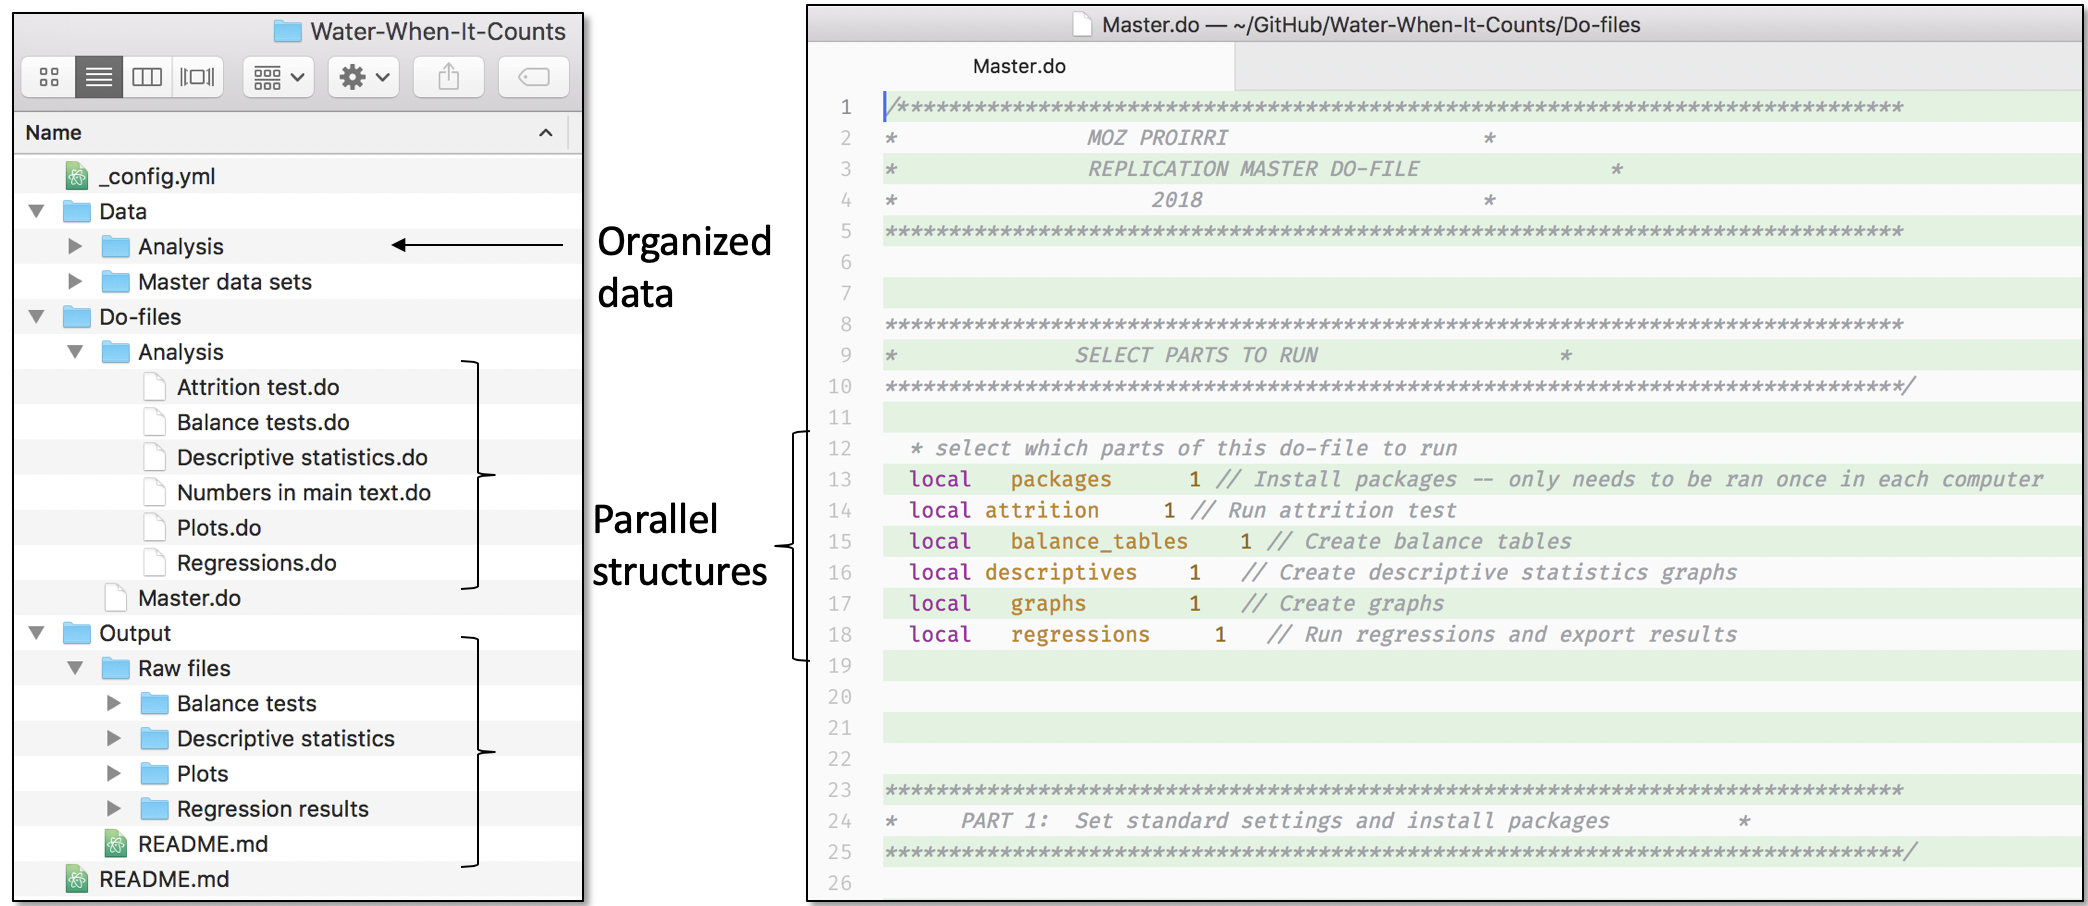
\includegraphics[width=\linewidth]{img/Organize2}
	\end{figure}

\end{frame}

%%%%%%%%%%%%%%% heading of section 1 %%%%%%%%%%%%%%%%%%%%
\sectionpic{Structure of the data folder}{img/section_slide}

\begin{frame}[fragile]{Dropbox (or equivalent) as Data Storage}
\begin{multicols}{2}	
	
	By the end of this presentation, you should understand how these two are connected in a research workflow:
	
	\begin{itemize}[<default overlay specification>]
		\item<1> \textbf{Privacy} - Personally-identified data is NEVER available to non-invited people (can be encrypted).
		\item<1> \textbf{Efficiency} - Only the most recent version of files is stored, and individuals can opt out of subfolders.
		\item<1> \textbf{Version Control } - Limited version control, but allows mistakes like deletions to be corrected quickly.
	\end{itemize}
	
	\begin{figure}
		\centering
		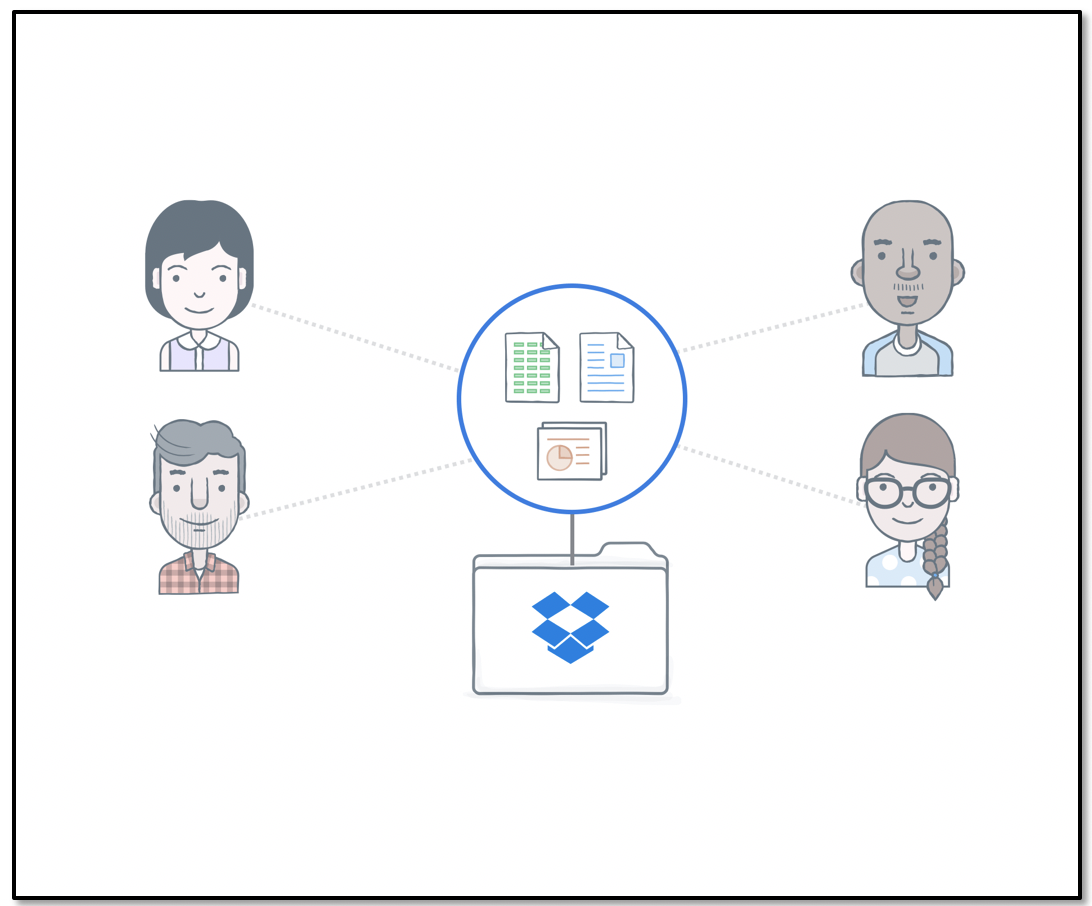
\includegraphics[width=50mm]{img/Structure}
	\end{figure}
	
\end{multicols}
\end{frame}

\begin{frame}[fragile]{Structure of the data folder: overview}
\begin{multicols}{2}	
	
	\textbf{The top-level data folder contains:}
	
	\begin{enumerate}[<default overlay specification>]
		\item<1> A folder for each analysis round (in this case, one folder each for baseline and endline).
		\item<1> An encrypted folder with keys to PII data (through software like TrueCrypt or BoxCrypt). 
		\item<1> A “master” file that traces all observations and linkages between data across rounds. 
	\end{enumerate}
	
	\begin{figure}
		\centering
		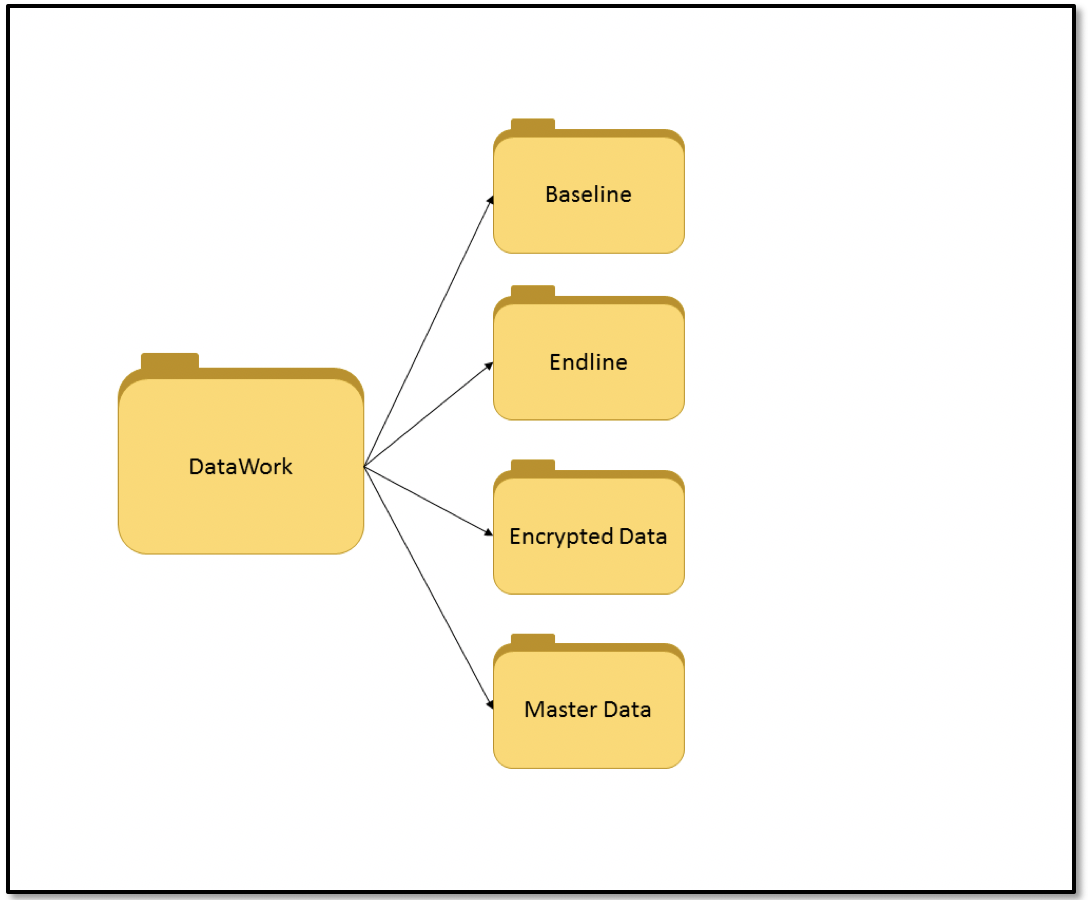
\includegraphics[width=50mm]{img/Structure2}
	\end{figure}
	
\end{multicols}
\end{frame}

\begin{frame}[fragile]{Structure of the data folder: the master file}
\begin{multicols}{2}	
	
	\begin{itemize}[<default overlay specification>]
		\item<1> Master data traces contacts across all rounds for analysis purposes that include analysis of loss to follow-up; differential attrition; and other key reporting elements of research design and execution. 
		\item<1> Every sampled unit that appears in every dataset here should be catalogued here across the whole project. 
	\end{itemize}
	
	\begin{figure}
		\centering
		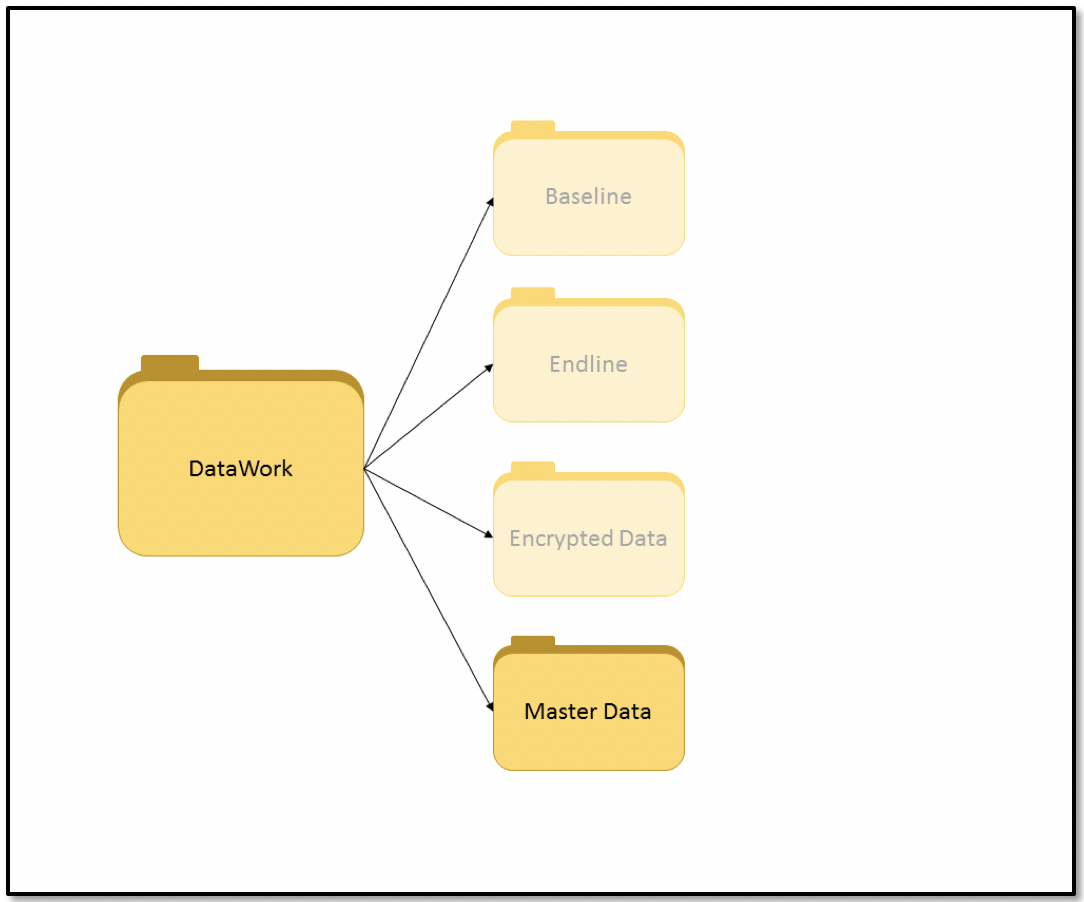
\includegraphics[width=50mm]{img/Structure3}
	\end{figure}
	
\end{multicols}
\end{frame}

\begin{frame}{Structure of the data folder: the master file}

	\begin{itemize}[<default overlay specification>]
	\item<1> Include all variables that are constant across the lifetime of a project in master data sets. 
			\newline - ID variables, treatment status, sampling dummies, monitor outcomes, geo-variables.
	\item<1> One master data set per unit of observation. 
	\item<1> Include all observations ever encountered – not just the observations you interview. 
	\item<1> If you have discrepancies across data sets, the master data set is the master. 
\end{itemize}

\end{frame}

\begin{frame}[fragile]{Structure of the data folder: encrypted data}
\begin{multicols}{2}	
	
	\begin{itemize}[<default overlay specification>]
		\item<1> The raw data with identifying information should be stored in the EncryptedData folder.
		\item<1> The do-files used to import your data from SurveyCTO or the equivalent software will also go in this folder. 
	\end{itemize}
	
	\begin{figure}
		\centering
		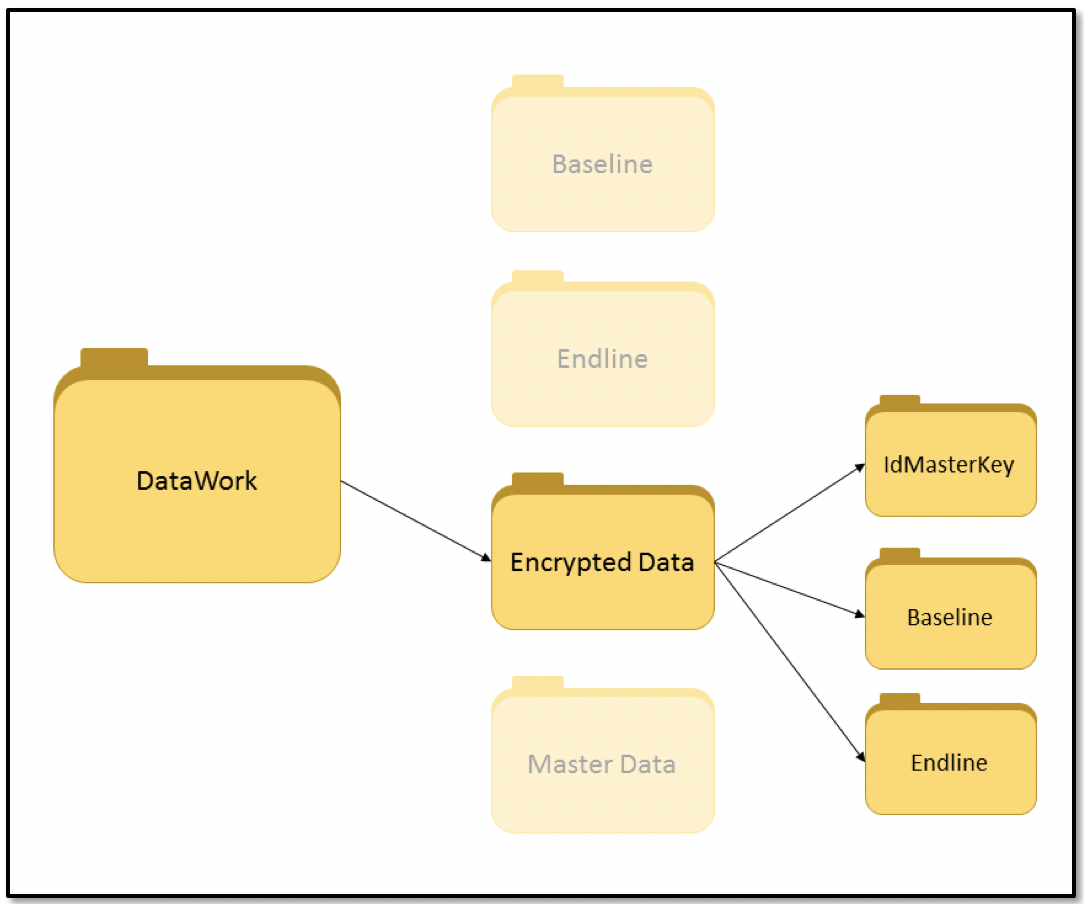
\includegraphics[width=50mm]{img/Structure4}
	\end{figure}
	
\end{multicols}
\end{frame}

\begin{frame}{Structure of the data folder: encrypted data}

	\begin{figure}
		\centering
		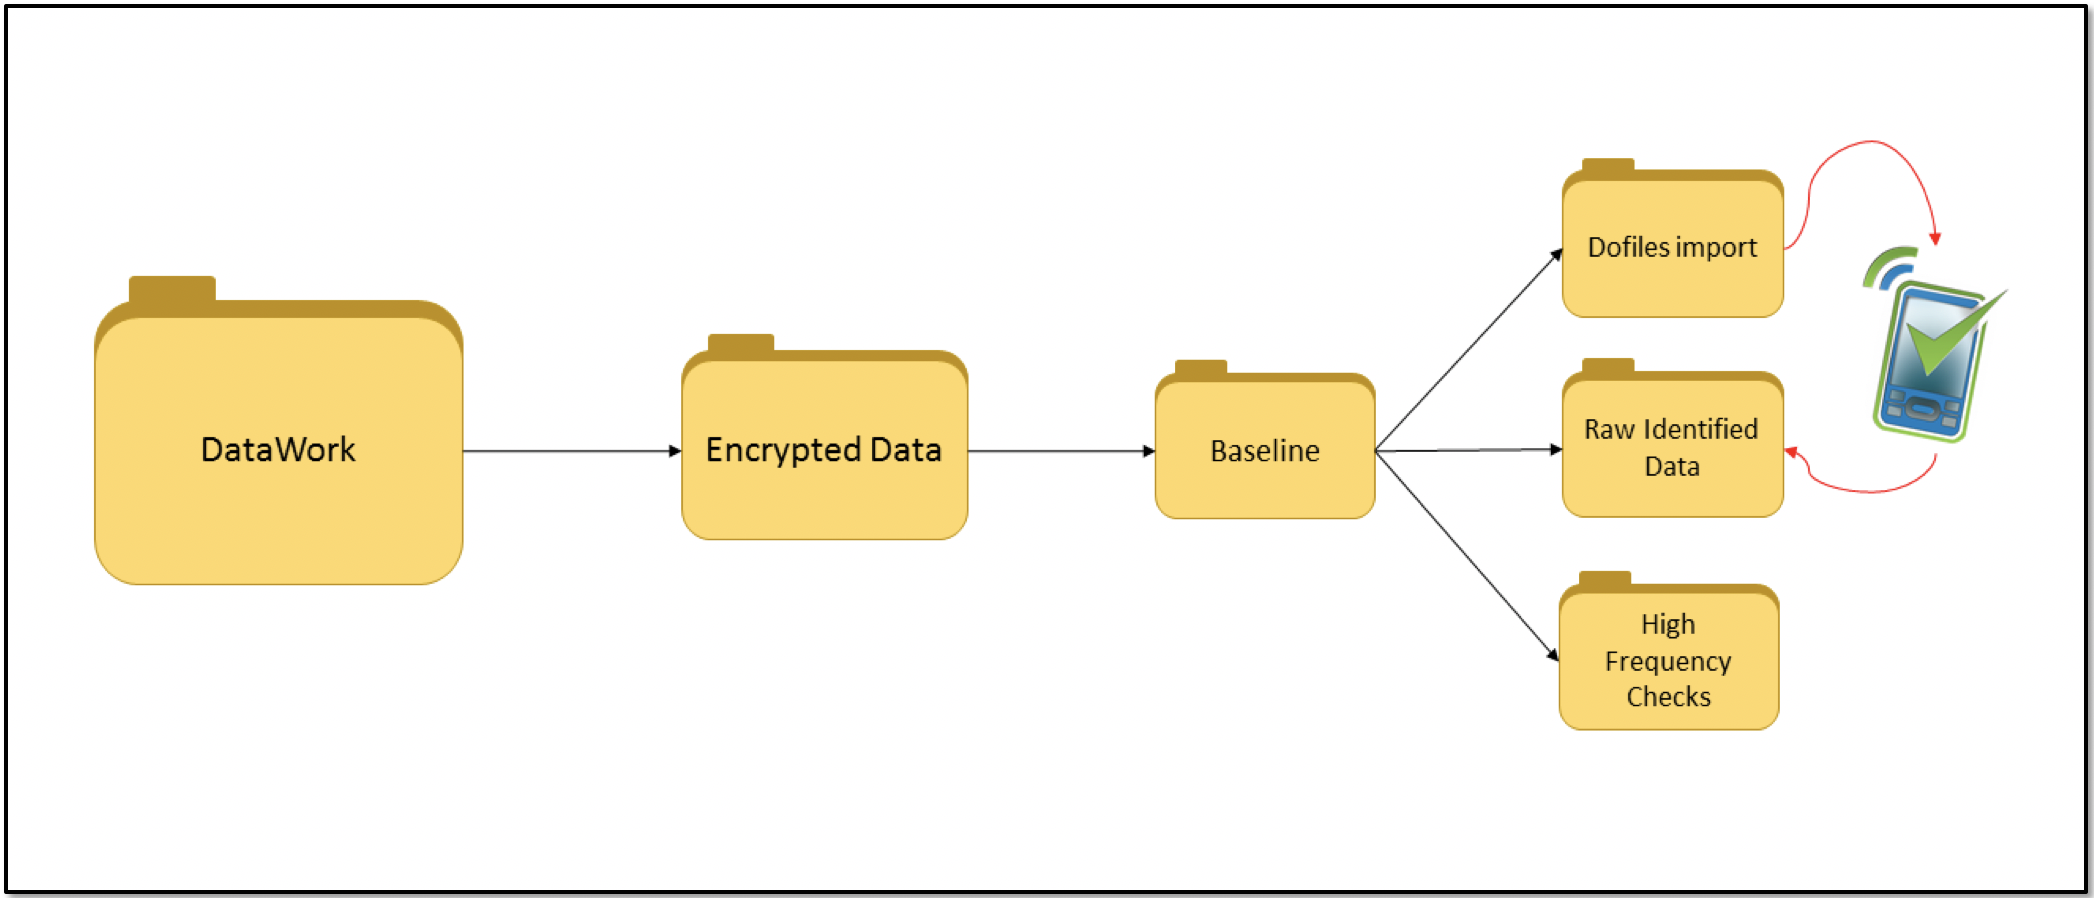
\includegraphics[width=\linewidth]{img/Structure5}
	\end{figure}

\end{frame}

\begin{frame}{Structure of the data folder: encrypted data}

	\begin{itemize}[<default overlay specification>]
	\item<1> Leave all files in this folder completely un-altered in the same format as you received them – guidance is forthcoming on a Boxcryptor license. 
	\item<1> As soon as you make a change to the data, correct any values, or even import it to a different format, save it somewhere else. 
	\item<1> Try to keep even file names unaltered. The exception is if you need to change the file name in order to be able to import them.
	\end{itemize}

\end{frame}


\begin{frame}{Structure of the data folder: analysis rounds}

	\begin{figure}
		\centering
		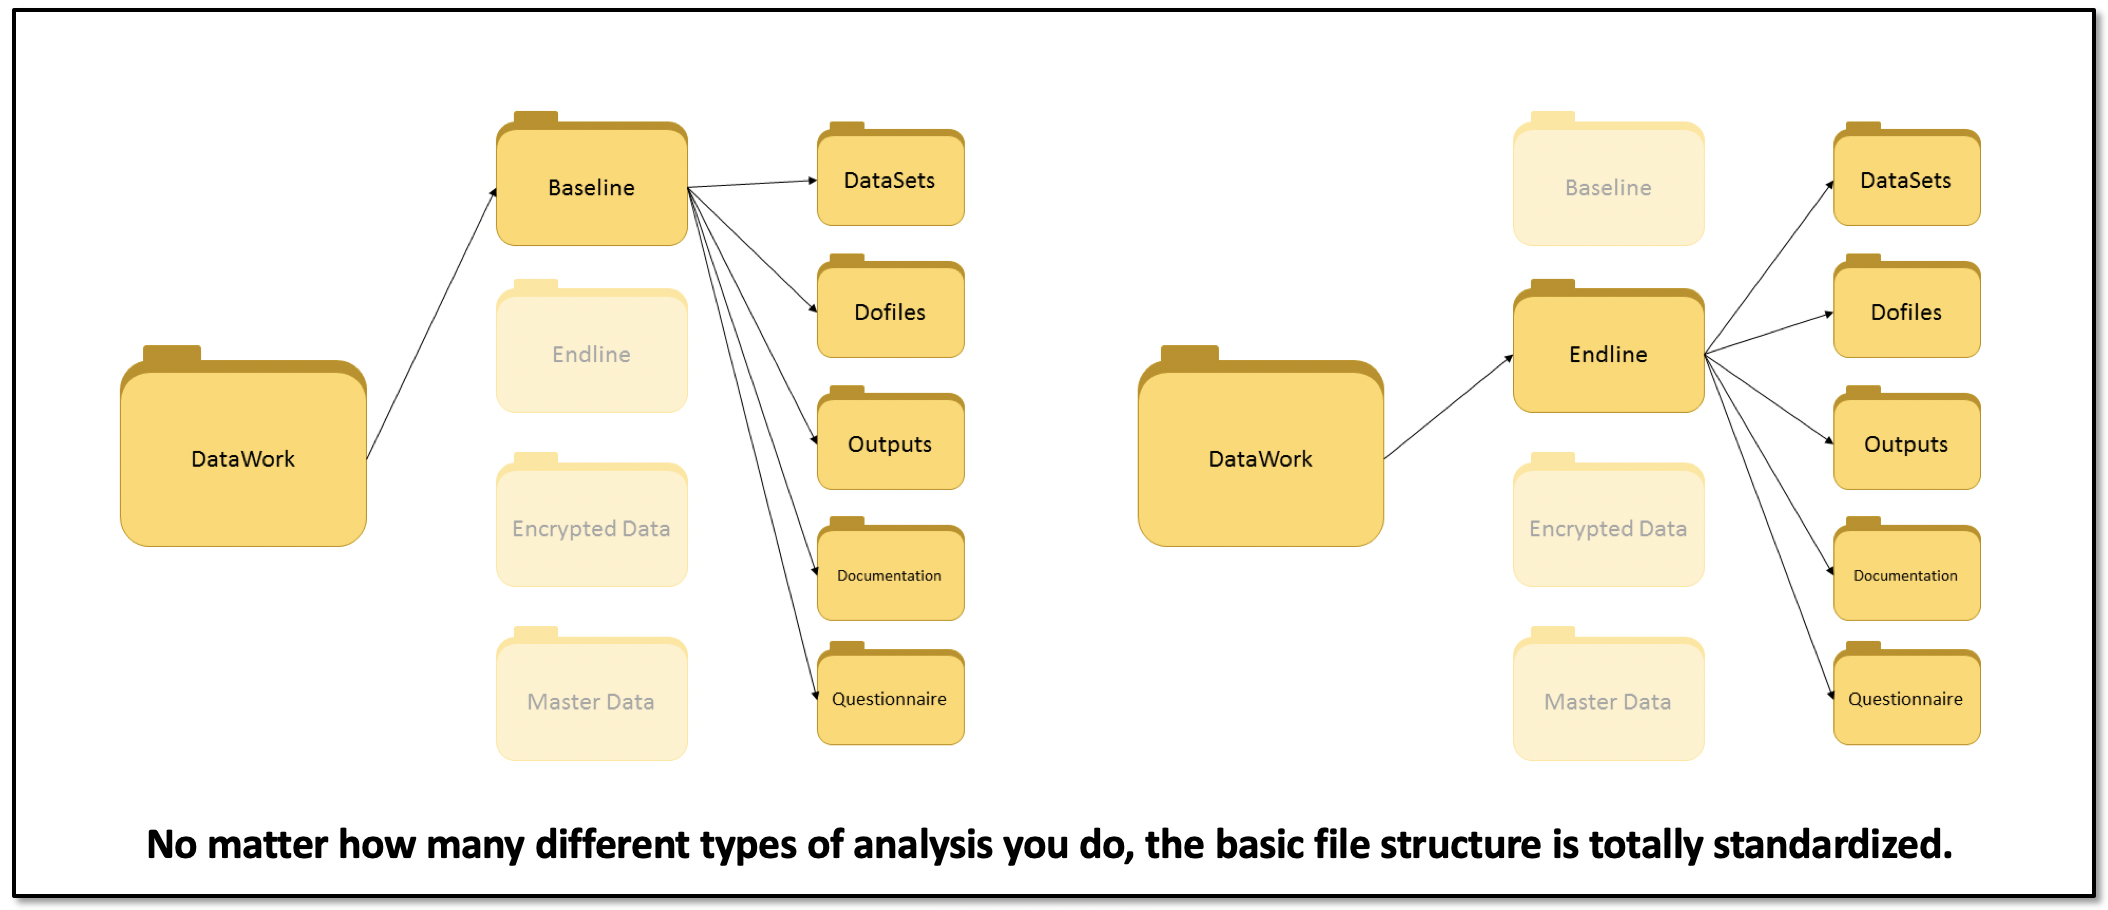
\includegraphics[width=\linewidth]{img/Structure6}
	\end{figure}

\end{frame}

%%%%%%%%%%%% heading of section 2 %%%%%%%%%%%%
\sectionpic{Structure of the analysis folders}{img/section_slide}

\begin{frame}{Structure of the analysis folder: overview}

	\begin{figure}
		\centering
		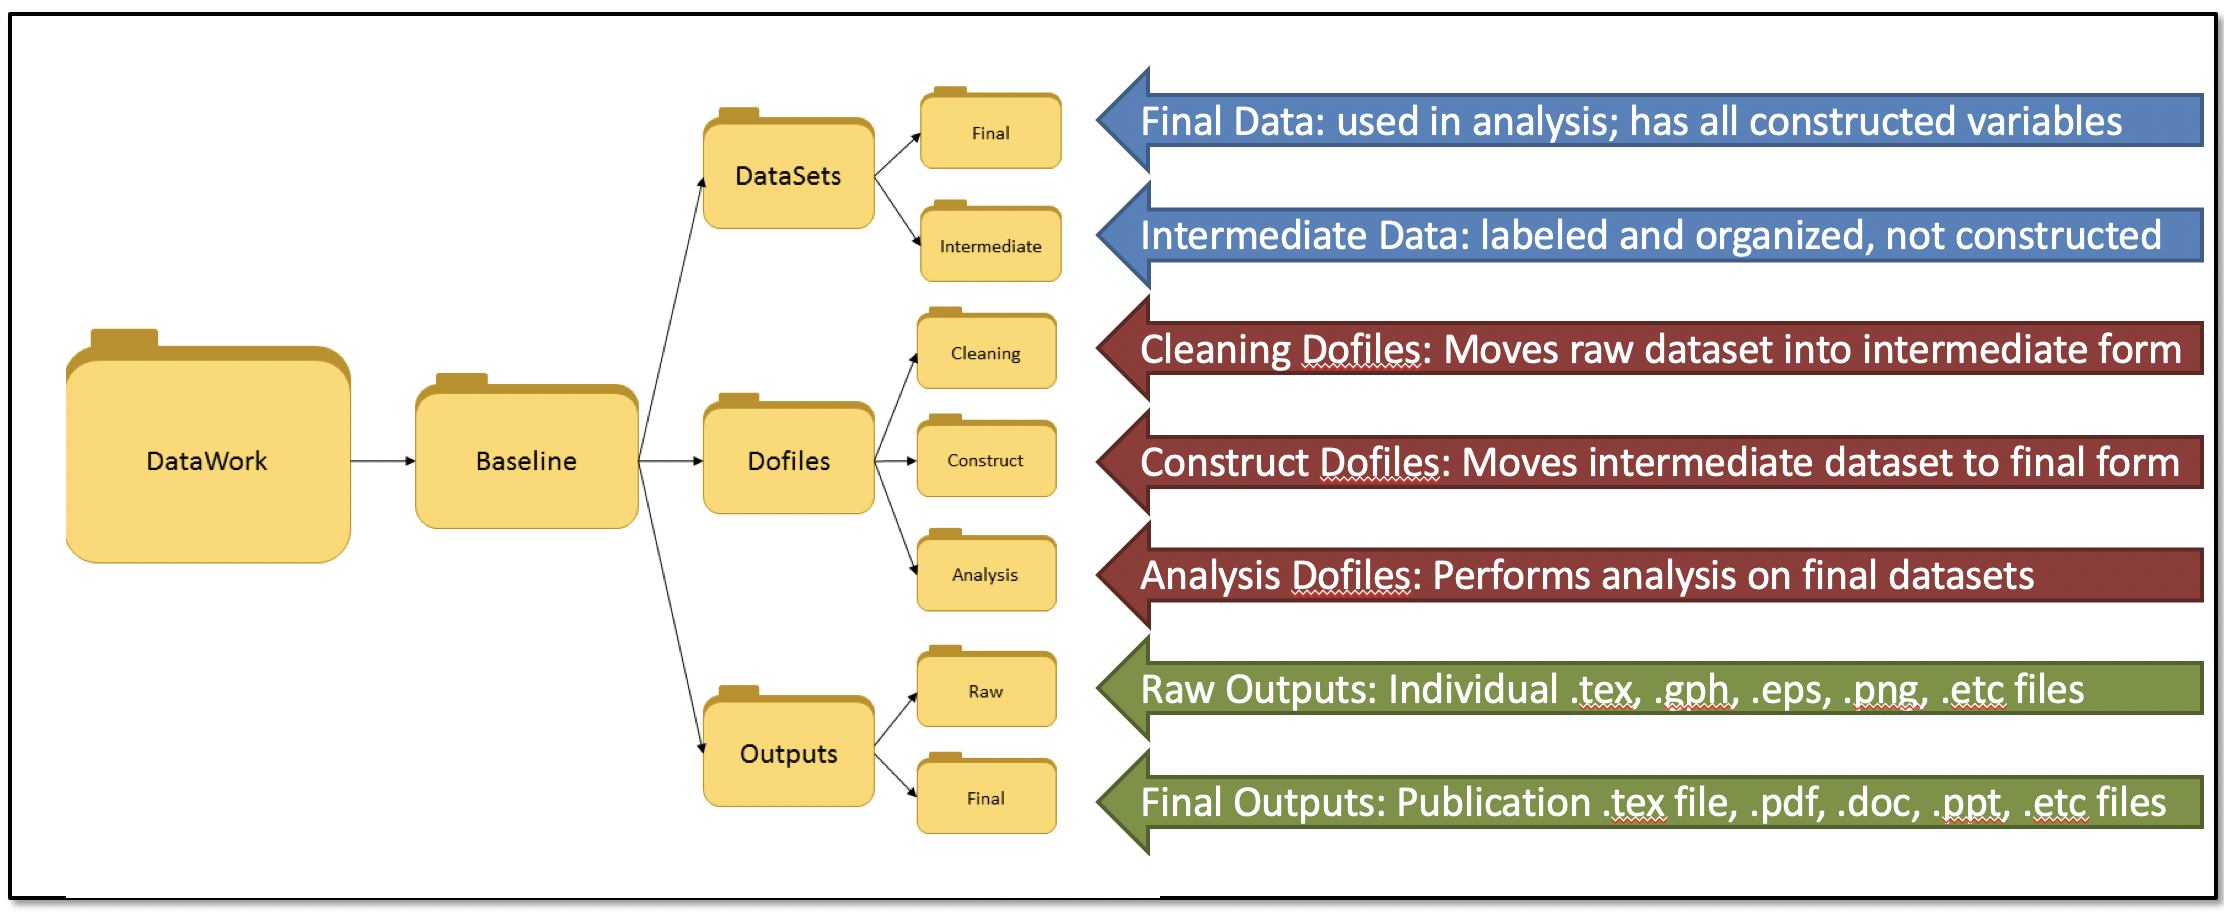
\includegraphics[width=\linewidth]{img/Structure7}
	\end{figure}

\end{frame}

\begin{frame}[fragile]{Structure of the analysis folder: cleaning data}
\begin{multicols}{2}	
	
	\textbf{The cleaning do-files will:}
	
	\begin{enumerate}[<default overlay specification>]
		\item<1> The raw data with identifying information should be stored in the EncryptedData folder.
		\item<1> The do-files used to import your data from SurveyCTO or the equivalent software will also go in this folder. 
		\item<1> Save as intermediate datasets
	\end{enumerate}
	
	\begin{figure}
		\centering
		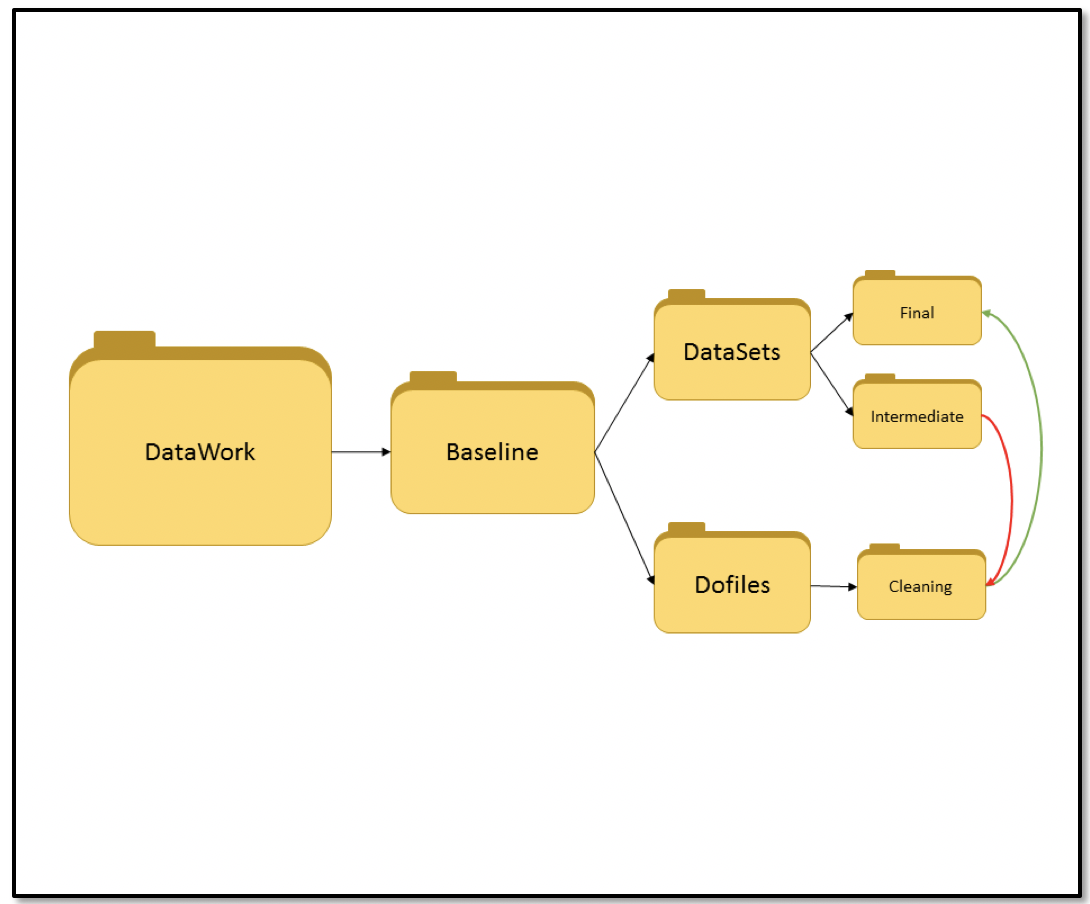
\includegraphics[width=50mm]{img/Structure8}
	\end{figure}
	
\end{multicols}
\end{frame}


\begin{frame}[fragile]{Structure of the analysis folder: cleaning data}
\begin{multicols}{2}	
	
	\textbf{The construct do-files will:}
	
	\begin{enumerate}[<default overlay specification>]
		\item<1> Load the intermediate data sets.
		\item<1> Create “constructed” variables for analysis. 
		\item<1> Save the final data sets in the Final DataSets folder
	\end{enumerate}
	
	Think of the “final” data as what would be released on Dataverse when the paper is published.
	
	\begin{figure}
		\centering
		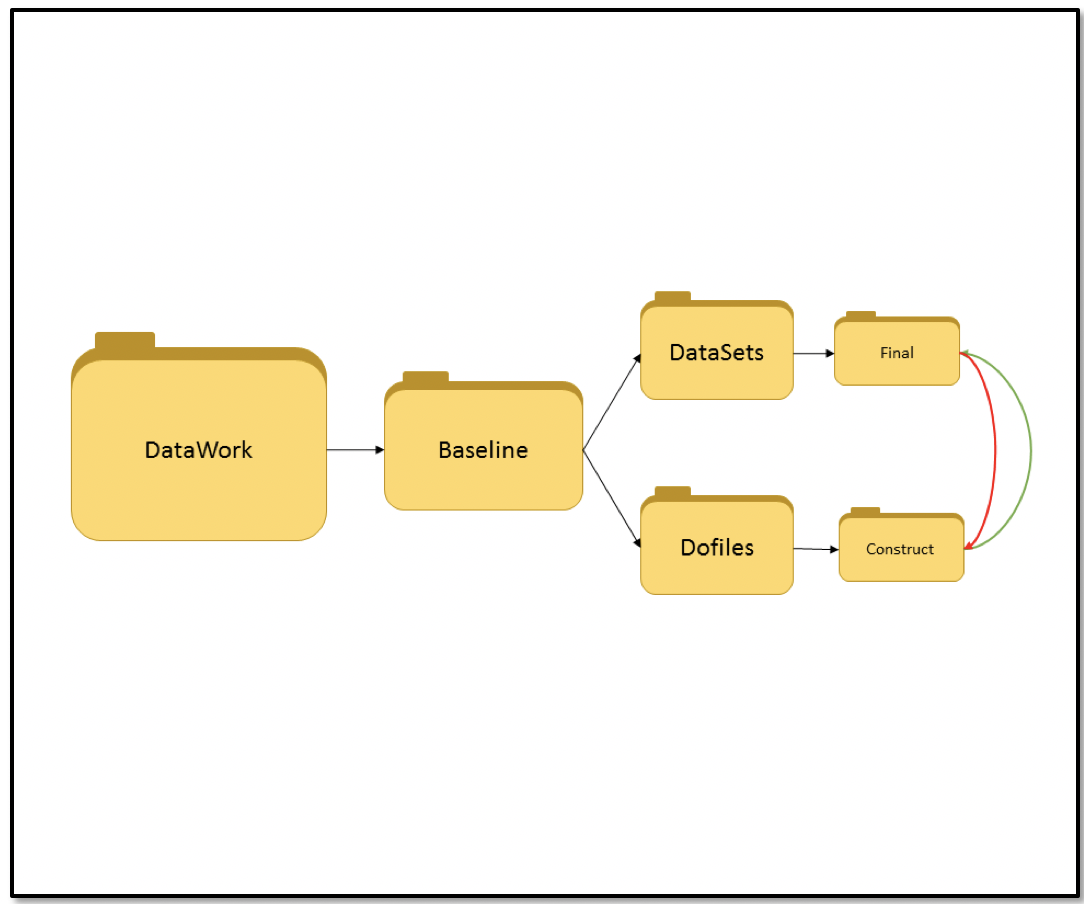
\includegraphics[width=50mm]{img/Structure9}
	\end{figure}
	
\end{multicols}
\end{frame}


\begin{frame}[fragile]{Structure of the analysis folder: analysis}
\begin{multicols}{2}	
	
	\textbf{The analysis do-files will:}
	
	\begin{enumerate}[<default overlay specification>]
		\item<1> Load the constructed data and run the analysis.
		\item<1> Outputs such as plots and tables generated by these do-files are stored in the Raw Outputs folder. 
		\item<1> Do not create variables in the analysis do-files!
		\item<1> Optionally the do-files themselves can be coded to push new outputs to GitHub/Overleaf and/or call pdflatex to compile new drafts.
	\end{enumerate}
	
	\begin{figure}
		\centering
		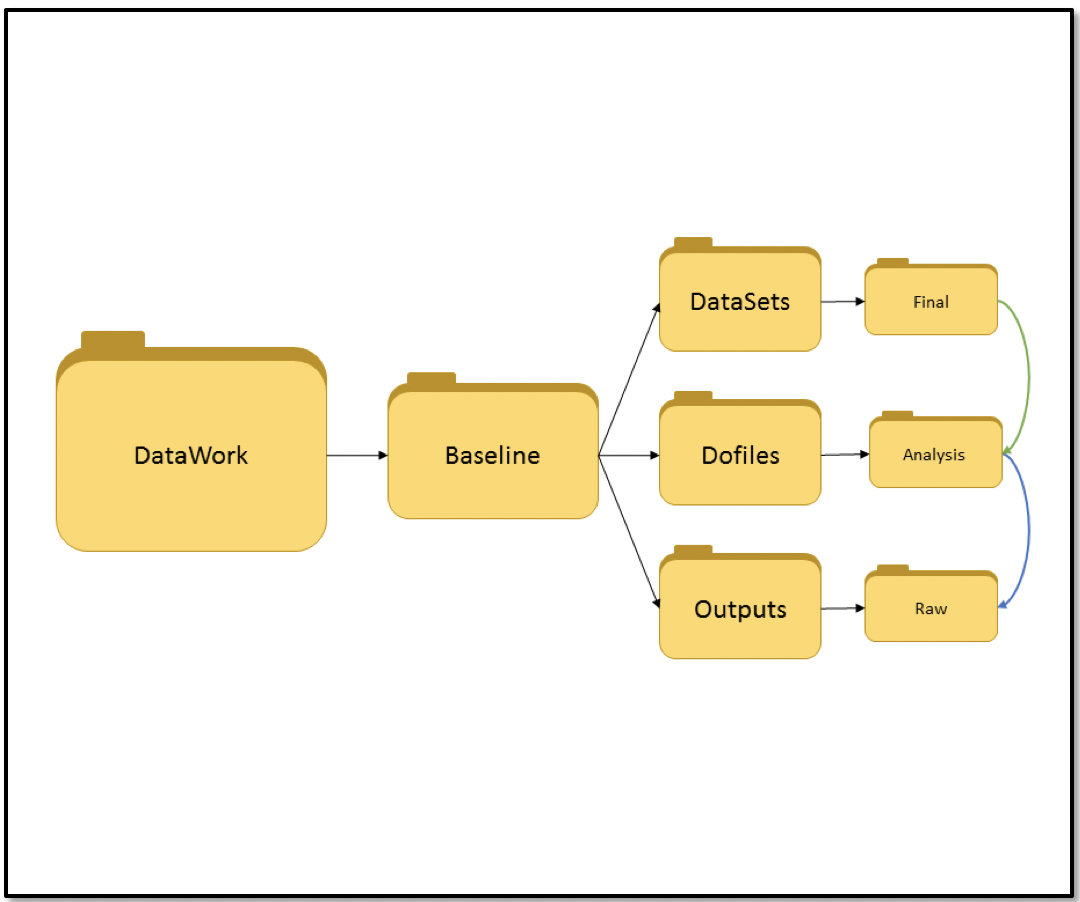
\includegraphics[width=50mm]{img/Structure10}
	\end{figure}
	
\end{multicols}
\end{frame}



\begin{frame}[fragile]{Structure of the analysis folder: outputs}
\begin{multicols}{2}	
	
	\textbf{The outputs folder will:}
	
	\begin{enumerate}[<default overlay specification>]
		\item<1> Hold “produced” materials that utilize the raw outputs (pdf documents, LaTeX documents, PowerPoints, Word, etc).
	\end{enumerate}
	
	\begin{figure}
		\centering
		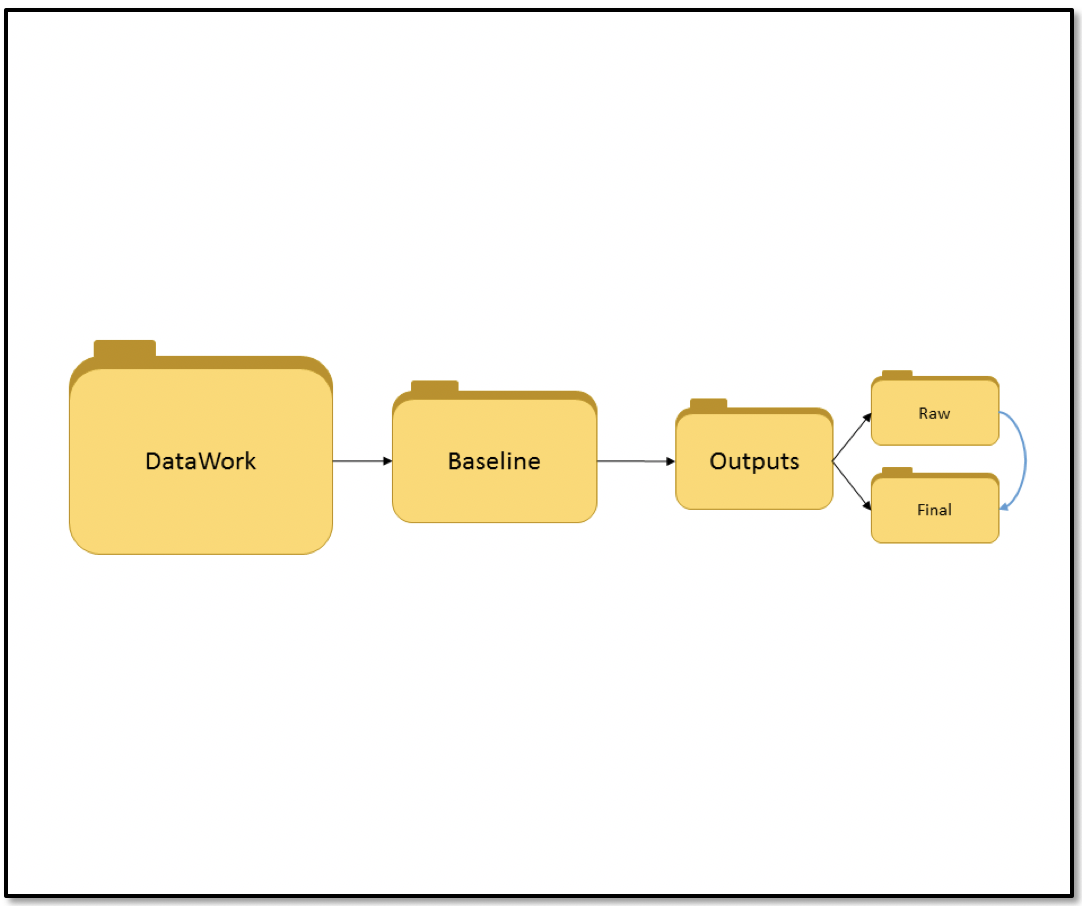
\includegraphics[width=50mm]{img/Structure11}
	\end{figure}
	
\end{multicols}
\end{frame}


\begin{frame}[fragile]{Structure of the analysis folder: outputs}
\begin{multicols}{2}	
	
	\textbf{The outputs folder will:}
	
	\begin{enumerate}[<default overlay specification>]
		\item<1> Once data collection is done, your project looks something like this.
		\item<1> Head on over to worldbank.github.io/ietoolkit
		\item<1> Or do \texttt{ssc install ietoolkit}.
		\item<1> Then, \texttt{iefolder} will set up your folders.
	\end{enumerate}
	
	\begin{figure}
		\centering
		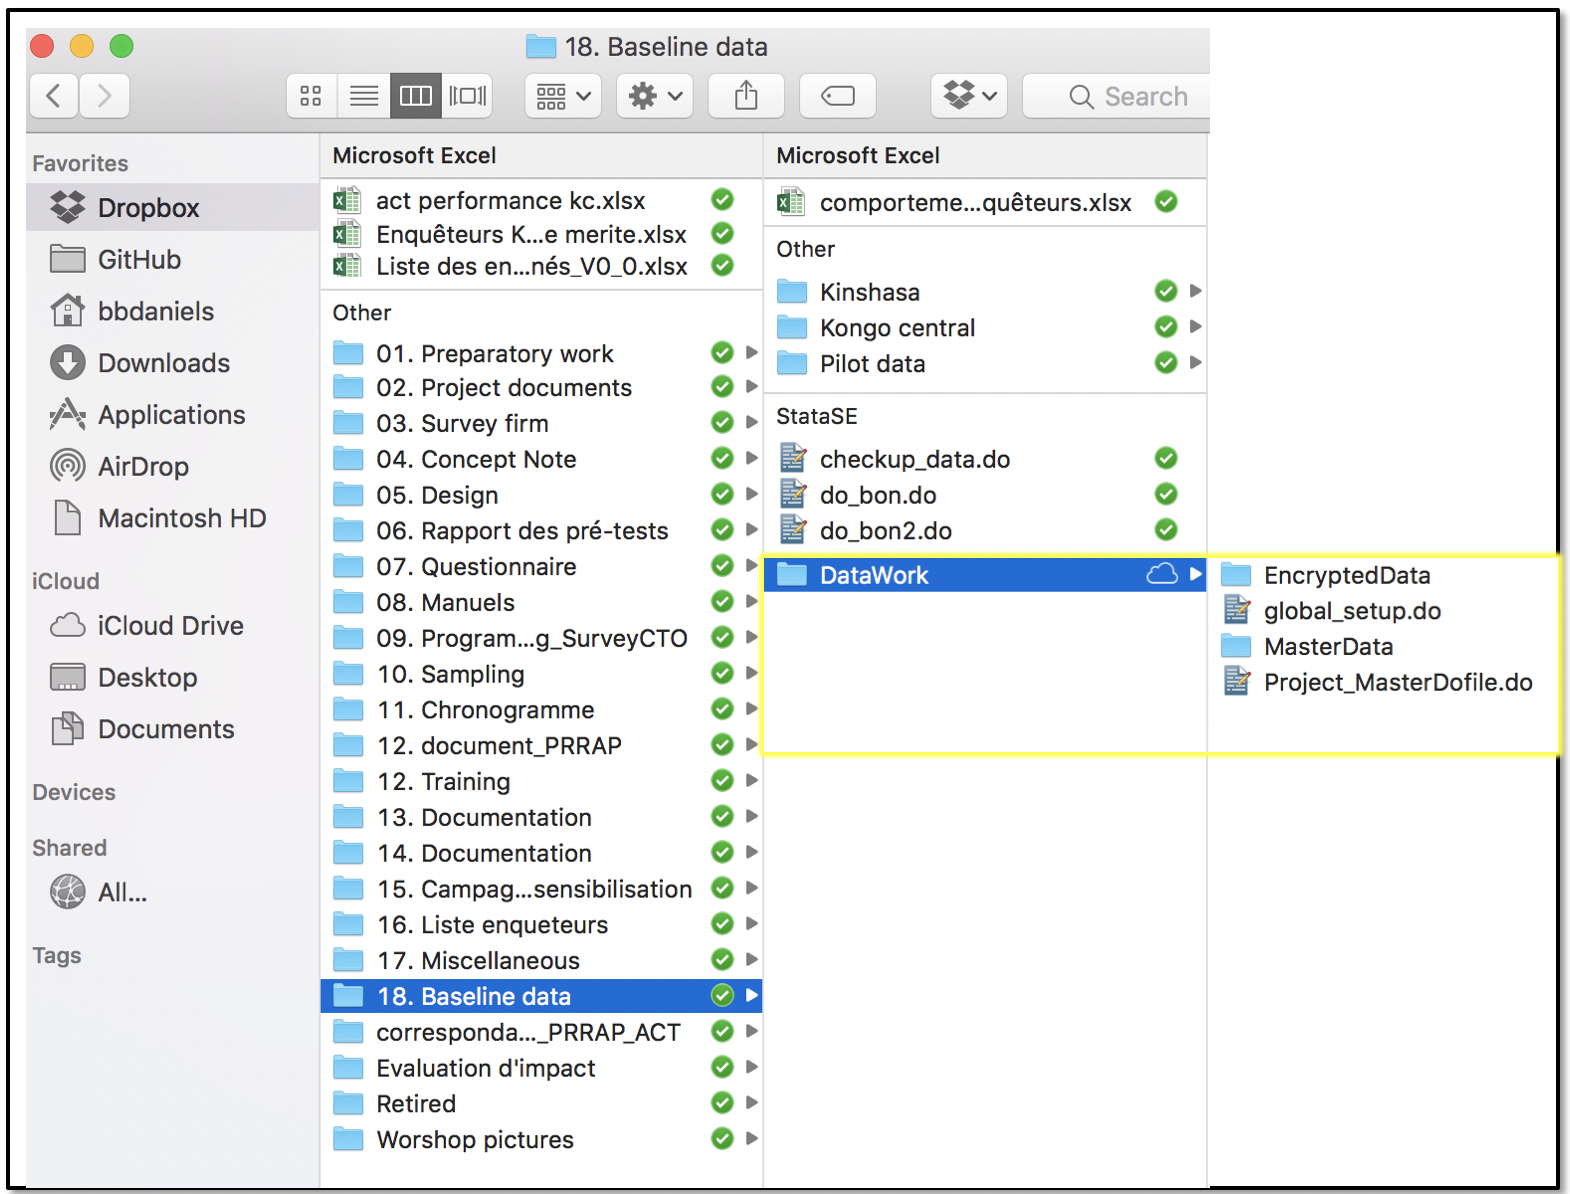
\includegraphics[height=55mm]{img/Structure12}
	\end{figure}
	
\end{multicols}
\end{frame}


%%%%%%%%%%%% heading of section 3 %%%%%%%%%%%%
\sectionpic{Master do-files provide structure}{img/section_slide}

\begin{frame}{Master do-files: overview}

	\begin{itemize}[<default overlay specification>]
		\item<1> \textbf{As you might have noticed, there are a lot of do-files in the workflow.}
			\newline - A big project can become very complex, and do-files need to be run in a certain order to create the right outputs.
			\newline - That could mean you’d need to write one extremely long do-file, or a different document with instructions about in which order to run all the do-files.
			\newline - Best to keep each dofile self-contained: some projects have one for every exhibit.
		\item<1> \textbf{So, you can make a do-file run other do-files using the [do] command.}
			\newline - This (and a few secondary but still important things) is what a master do-file does.
			\newline - The master do-file is the map over all data work in your data folder.
			\newline - It’s the table of contents for the instructions that you code.
			\newline - A total stranger who wants to replicate all your work should only have to open this one short dofile to have a complete roadmap of the analysis.
	\end{itemize}

\end{frame}


\begin{frame}[fragile]{Master do-files: Intro header}
\begin{multicols}{2}	
	
	\begin{itemize}[<default overlay specification>]
		\item<1> Short descriptives in the file allow a reader to get the gist of what is accomplished, whether they are reading the right code, and anything else needed.
		\item<1> Highlights key information about the dataset, such as unique ID.
		\item<1> Details outputs created and explains how any outputs not included are created (by hand, with confidential data, etc).
	\end{itemize}
	
	\begin{figure}
		\centering
		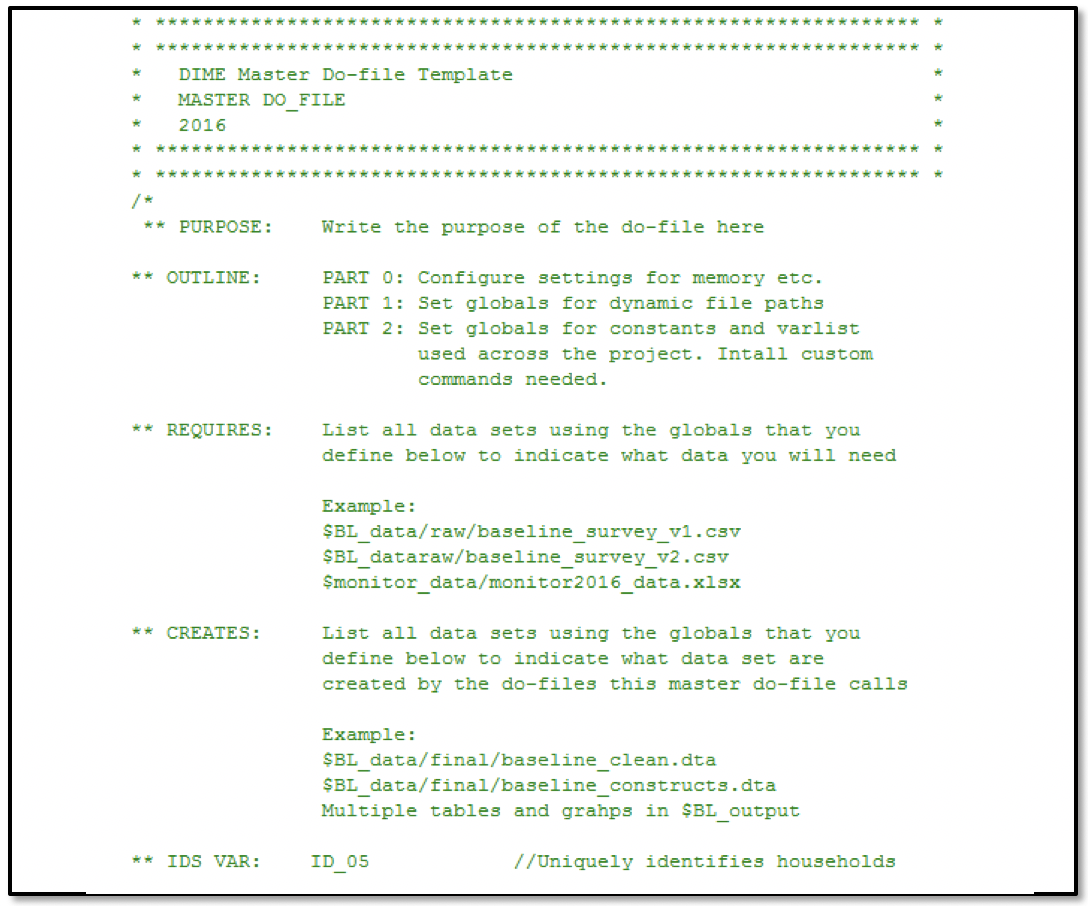
\includegraphics[height=55mm]{img/Structure13}
	\end{figure}
	
\end{multicols}
\end{frame}


\begin{frame}[fragile]{Master do-files: Default settings}
\begin{multicols}{2}	
	
	\begin{itemize}[<default overlay specification>]
		\item<1> These commands make everyone’s life easier by disabling some of Stata’s annoying defaults.
		\item<1> ”version” command is essential:
			\newline - Changes to version can alter the results of randomizations.
			\newline - Some commands will break on newer/older versions due to changes in syntax.
	\end{itemize}
	
	\begin{figure}
		\centering
		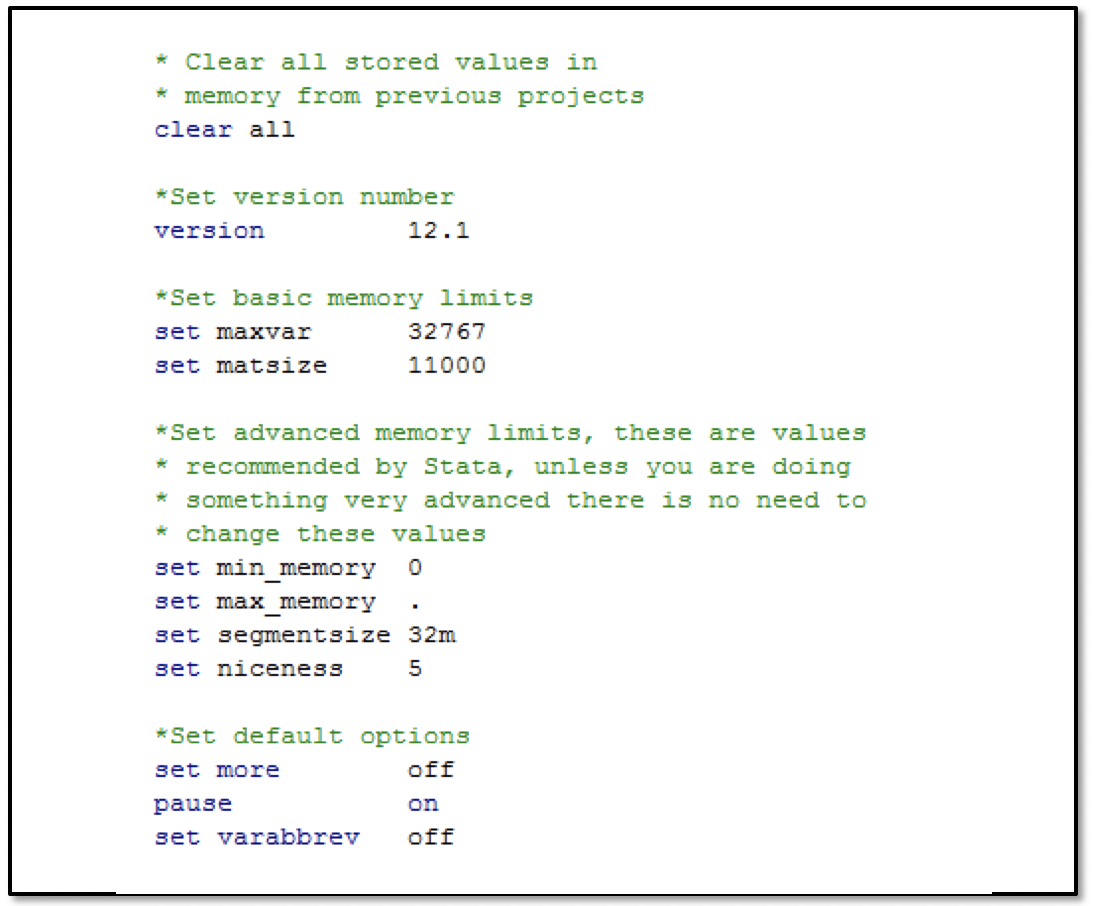
\includegraphics[height=55mm]{img/Structure14}
	\end{figure}
	
\end{multicols}
\end{frame}


\begin{frame}[fragile]{Master do-files: Folder paths}
\begin{multicols}{2}	
	
	\begin{itemize}[<default overlay specification>]
		\item<1> This crucial component allows a new user to point the entire analysis at the correct (cloned or synced) iteration of the folder.
		\item<1> If this is not available, new users will spend a long time changing filepaths scattered throughout the dofiles.
		\item<1>  ALWAYS USE \texttt{"/"} 
	\end{itemize}
	
	\begin{figure}
		\centering
		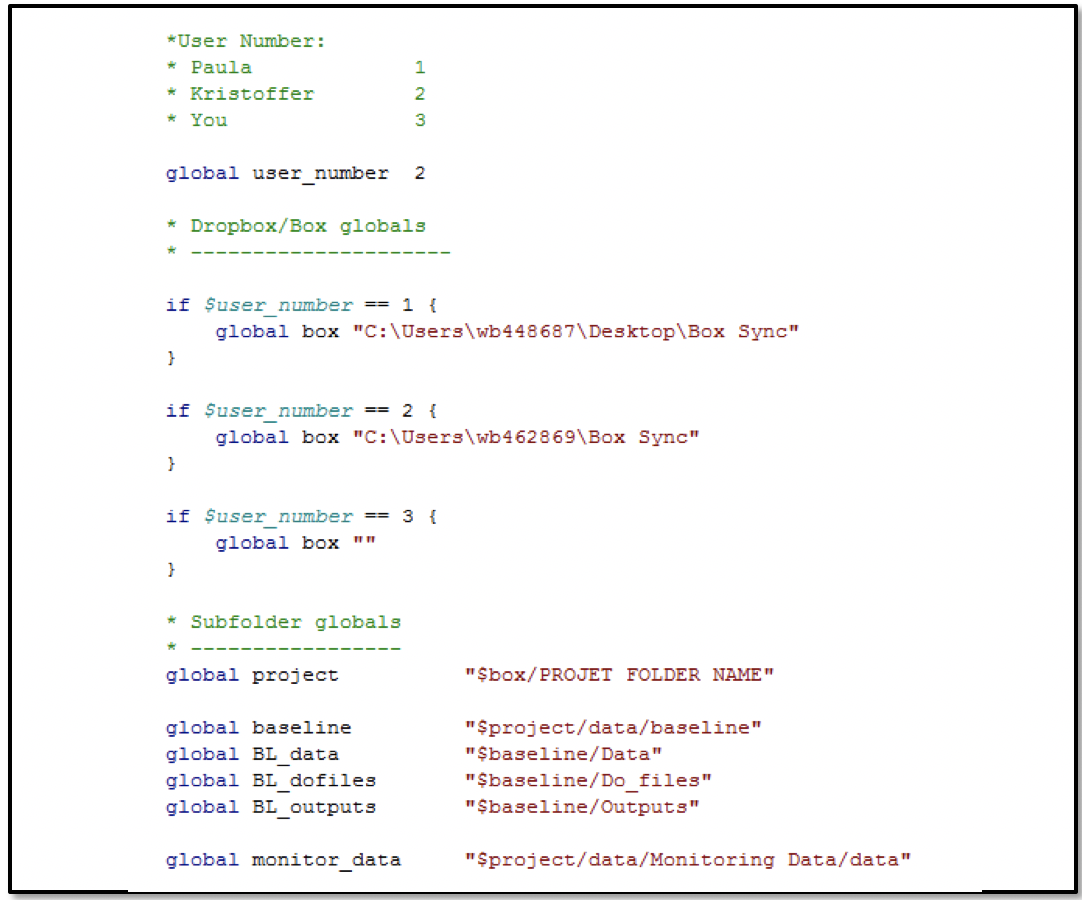
\includegraphics[height=55mm]{img/Structure15}
	\end{figure}
	
\end{multicols}
\end{frame}


\begin{frame}[fragile]{Master do-files: Globals and programs}
\begin{multicols}{2}	
	
	\begin{itemize}[<default overlay specification>]
		\item<1> Add conversions that are needed for the analysis.
		\item<1> Add controls lists that are used throughout the paper, so that all regressions can be altered correctly with one line.
		\item<1>  Add options (such as graphing options, clustering, etc). 
		\item<1>  Any external programs that need to be installed for code to run.
	\end{itemize}
	
	\begin{figure}
		\centering
		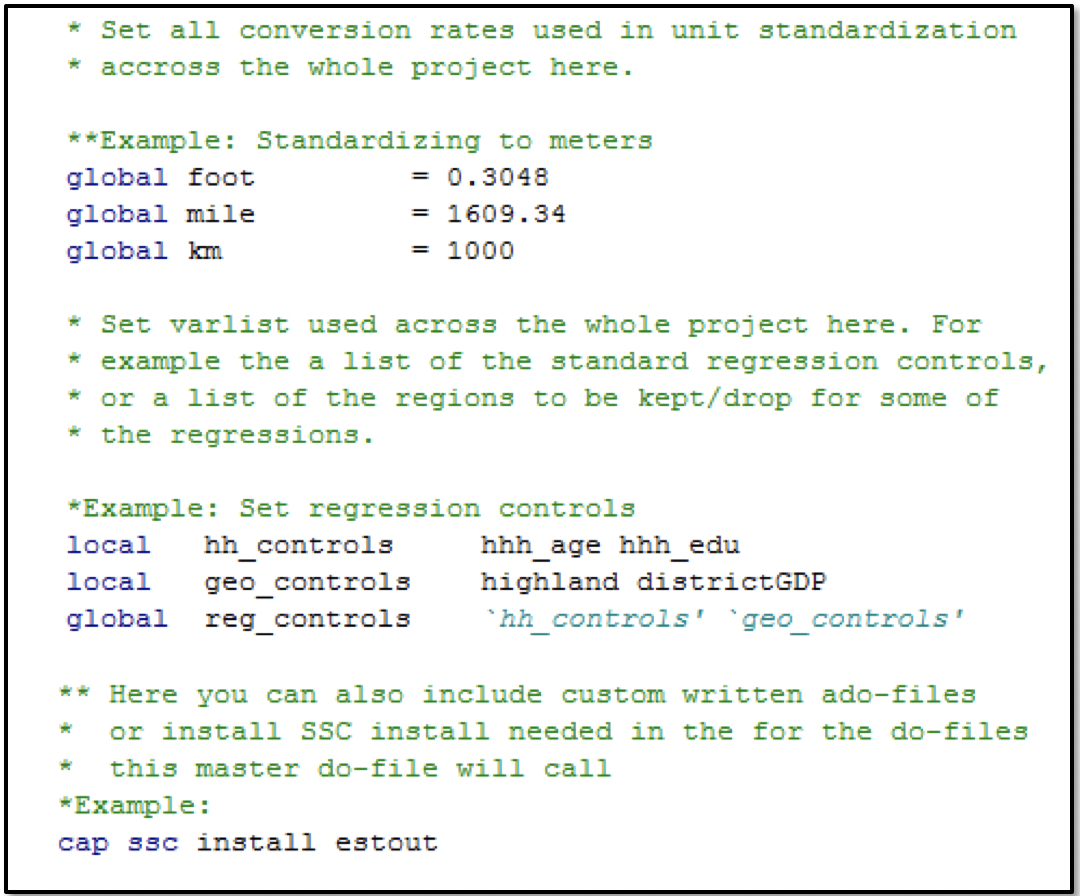
\includegraphics[height=55mm]{img/Structure16}
	\end{figure}
	
\end{multicols}
\end{frame}

\begin{frame}[fragile]{Master do-files: Actually doing stuff}
\begin{multicols}{2}	
	
	\begin{itemize}[<default overlay specification>]
		\item<1> Detail what each file called in the master do-file is responsible for.
		\item<1> If there are a lot of do-files, create a sub-master for each high level task 
		\item<1> Use comments that explain where in your code you do what. 
	\end{itemize}
	
	\begin{figure}
		\centering
		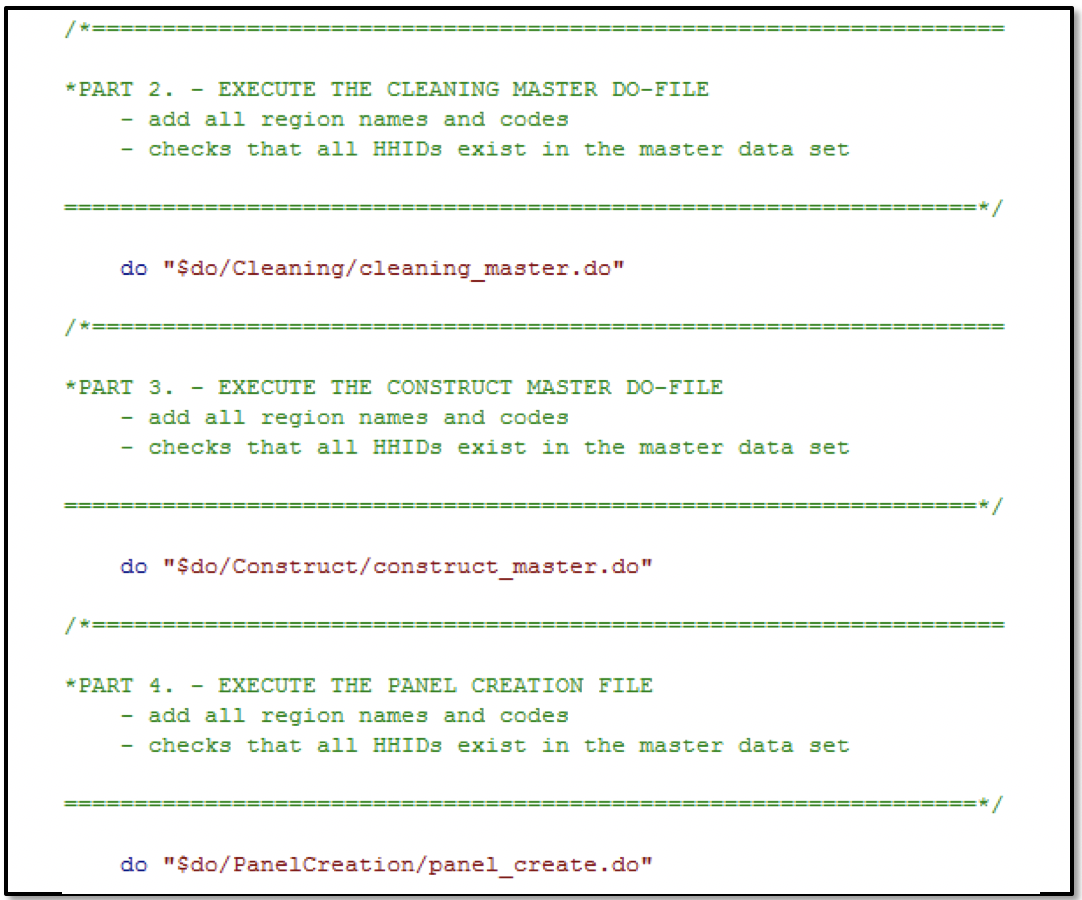
\includegraphics[height=55mm]{img/Structure17}
	\end{figure}
	
\end{multicols}
\end{frame}

%%%%%%%%%%%%%%%%%%%%%%%%%%%%%%%%%%%%%%%%%%% Final thougts section
\begin{frame}{Conclusion}

Thank You!

\vspace{20mm}
For more information or further questions please contact:
\newline Benjamin Daniels  (\url{bdaniels@worldbank.org }) 

\end{frame}

%%%%%%%%%%%%%%%%%%%%%%%%%%%%%%%%%%%%%%%%%%% The End
\sectionpic{The End}{img/section_slide}






\end{document} 